\documentclass{beamer}
\mode<presentation>
{
  \usetheme{default}      % or try Darmstadt, Madrid, Warsaw, ...
  \usecolortheme{default} % or try albatross, beaver, crane, ...
  \usefonttheme{default}  % or try serif, structurebold, ...
  \setbeamertemplate{navigation symbols}{}
  \setbeamertemplate{caption}[numbered]
} 

\usepackage[english]{babel}
\usepackage[utf8x]{inputenc}
\usepackage{scrextend}
\usepackage{graphicx}
\usepackage{booktabs}
\usepackage{adjustbox}
\usepackage{marvosym}
\graphicspath{ {./images/} }

\title[Pres]{Integrating Logical Dependencies in Software Clustering:\\ A Case Study on Apache Ant}
\author{Adelina Stana \and Ioana Şora}
\institute{Computer Science and Engineering Department\\
"Politehnica" University of Timișoara, Romania}
\date{}

\begin{document}

\begin{frame}
  \titlepage
\end{frame}

% Uncomment these lines for an automatically generated outline.
\begin{frame}{Outline}
  \tableofcontents
\end{frame}

\section{Introduction}

\begin{frame}
\frametitle{Introduction}
\begin{itemize}
    \item Software architecture helps developers understand the system and its behavior.
    \item Architectural reconstruction is needed when documentation is missing or outdated.
    \item Software clustering is used to identify modules or subsystems for reconstruction.
    \item Logical dependencies, extracted from co-changes in versioning systems, can provide additional insights.
\end{itemize}
\end{frame}

\section{Motivation}

\begin{frame}
\frametitle{Motivation}
\begin{itemize}
    \item Previous research shows logical dependencies are distinct from structural dependencies.
    \item Incorporating logical dependencies may improve software clustering results.
    \item Aim: Analyze the impact of logical dependencies on clustering solutions.
\end{itemize}
\end{frame}

\section{Logical Dependencies}

\begin{frame}
\frametitle{Logical Dependencies}
\begin{block}{Definition}
Logical dependencies are relationships between software entities identified by analyzing co-changes in the versioning system, representing functional dependencies not evident from code analysis.
\end{block}

\begin{center}
     \begin{figure}
    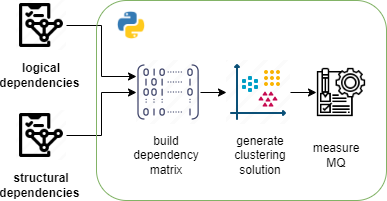
\includegraphics[width=0.8\textwidth]{clustering-generation.png}
    \caption{Clustering solution creation process diagram}
    \label{fig:clustering-gen}
     \end{figure}
\end{center}
\end{frame}

\begin{frame}
\frametitle{Metrics for Logical Dependencies}
\begin{itemize}
    \item \textbf{Support}: Frequency of updates where entities A and B change together.
    \item \textbf{Confidence}: Proportion of co-changes relative to total updates of an entity.
    \item \textbf{Strength}: Adjusted confidence metric that accounts for the system's average number of updates.
\end{itemize}
\end{frame}

\section{Related Work}

\begin{frame}
\frametitle{Related Work}
\begin{itemize}
    \item Software clustering often uses structural dependencies from code.
    \item Other approaches use lexical dependencies or co-change data.
    \item Evaluation metrics like MOJO and Modularization Quality (MQ) are used to assess clustering results.
\end{itemize}
\end{frame}

\section{Methodology}

\begin{frame}
\frametitle{Methodology Overview}
\begin{itemize}
    \item Case study on Apache Ant.
    \item Three scenarios:
    \begin{enumerate}
        \item Clustering using structural dependencies only.
        \item Clustering using logical dependencies only.
        \item Clustering using both logical and structural dependencies.
    \end{enumerate}
    \item Use of Louvain Clustering algorithm.
    \item Evaluation using Modularization Quality (MQ) metric.
\end{itemize}
\end{frame}

\begin{frame}
\frametitle{Clustering Generation Process}
\begin{center}
     \begin{figure}
    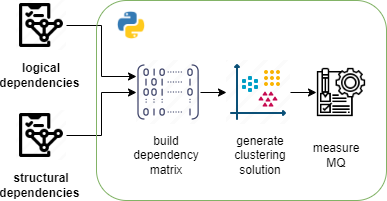
\includegraphics[width=0.8\textwidth]{clustering-generation.png}
    \caption{Clustering solution creation process diagram}
    \label{fig:clustering-gen}
     \end{figure}
\end{center}
\end{frame}

\begin{frame}
\frametitle{Louvain Clustering Algorithm}
\begin{itemize}
    \item Community detection algorithm for complex networks.
    \item Optimizes modularity by moving nodes between clusters.
    \item Suitable for large-scale clustering tasks.
\end{itemize}
\end{frame}

\section{Results}

\begin{frame}
\frametitle{Clustering Results}
\begin{center}
    \begin{table}
    \centering
    \caption{Louvain Clustering Results}
    \begin{tabular}{lccc}
        \toprule
        \textbf{Dataset} & \textbf{Entities} & \textbf{Clusters} & \textbf{MQ Metric} \\
        \midrule
        SD only & 517 & 12 & 0.08 \\
        LD only (Strength 30\%) & 174 & 44 & 0.558 \\
        SD + LD (Strength 30\%) & 517 & 15 & 0.227 \\
        \bottomrule
    \end{tabular}
    \end{table}
\end{center}
\end{frame}

\section{Discussion}

\begin{frame}
\frametitle{Analysis of Results}
\begin{itemize}
    \item Incorporating logical dependencies improves MQ scores.
    \item Clusters are more cohesive and functionally meaningful.
    \item Detailed analysis of specific classes demonstrates the benefits.
\end{itemize}
\end{frame}


\section{Conclusion}

\begin{frame}
\frametitle{Conclusion}
\begin{itemize}
    \item Incorporating logical dependencies improves clustering quality.
    \item Provides additional insights not available from code analysis alone.
    \item The combined approach leads to clusters that better reflect the system's architecture.
\end{itemize}
\end{frame}

\section{Future Work}

\begin{frame}
\frametitle{Future Work}
\begin{itemize}
    \item Expand analysis to more projects.
    \item Explore alternative evaluation metrics.
    \item Further investigate the role of logical dependencies in software clustering.
\end{itemize}
\end{frame}

\end{document}
